\documentclass[11pt]{article}

  \usepackage{fullpage}
  \usepackage{graphicx}
  \graphicspath{ {./images/} }
  \setlength{\parindent}{0pt} 
  \setlength{\parskip}{1em}



  \begin{document}
  \title{ARM Final Report}
  \author{Otto White, Paulo Lemos, Robert Stok, Weizhong Zhao}

  \maketitle

  \section*{Assembler Structure and Implementation}

  \begin{figure}[h]
  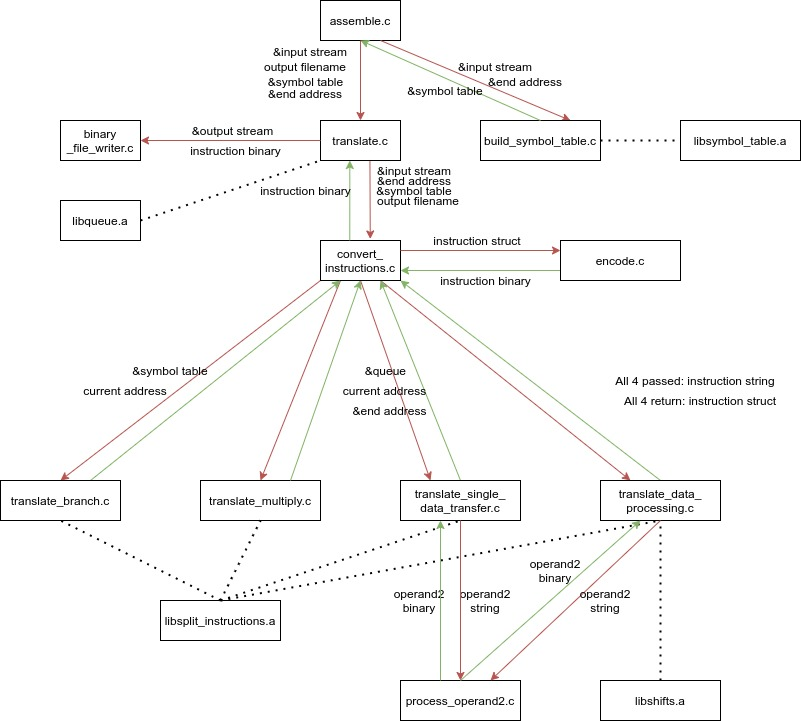
\includegraphics[scale=0.3]{assembler_structure}
  \centering
  \end{figure}

The assembler is structured as follows:

\begin{itemize}
\item \texttt{assemble.c} contains the main function which takes the input and output filenames as arguments; the input file contains ARM11 assembly instructions and the output file will have assembled ARM11 binary code written to it. Main calls build\_symbol\_table from \texttt{build\_symbol\_table.c} which passes through the input file once. After rewinding the input file to the original file position, translate from \texttt{translate.c} is called for the second pass. Finally, the memory allocated to symbol table is freed to prevent memory leaks.

\item \texttt{build\_symbol\_table.c} defines the build\_symbol\_table function which creates a node-based linked list mapping labels to memory addresses from label assignment instructions found in the input file. Each node struct has memory dynamically allocated and stores a label, an address and a pointer to the next node. Various helper functions and the struct definition are in symbol\_table.c in the \texttt{utilities} folder. In particular, the search\_table function is useful for retrieving the memory address when given a label. The head node is returned by build\_symbol\_table.

\item \texttt{translate.c} defines the translate function which reads the input file line by line. Next, each line is passed to convert\_instructions in \texttt{convert\_instructions.c} and then written to the output file with binary\_file\_writer in \texttt{utilities}.

\item \texttt{convert\_instructions.c} defines the convert\_instructions function. First, this determines the nature of an instruction and passes it to the appropiate function from translate\_multiply, translate\_single\_data\_transfer, translate\_branch or translate\_data\_processing. The output is then fed through encode in \texttt{encode.c} and returned.

\item \texttt{translate\_multiply.c, translate\_single\_data\_ transfer.c, translate\_branch.c,} \\ \texttt{translate\_data\_processing.c} each define the respective translate functions. A common tokenizer in split\_instructions.c in \texttt{utilities} is used to seperate the instruction and avoid code duplication. A new Instruction struct, representing the instruction, is populated with relevant opcodes and operand fields and then returned.

\item \texttt{encode.c} defines the encode function which builds the final binary word from the instruction struct and returns it as a uint\_32t.

\item \texttt{definitions.h} contains the Instruction\_Type, Condition and Opcode enum and Instruction struct definitions.

\item \texttt{utilities} contains binary\_file\_writer, split\_instructions(tokenizer), symbol\_table and miscellaneous helper functions for specific instruction translation functions.

\item \texttt{testing} contains unit tests for different parts of the assembler.

\end{itemize}


  \section*{Extension}

  \subsection*{Overview of the Extension}
  For our extension we created a machine vision library to efficiently transform images and videos. Using this library we then implemented a background removal program using edge detection and bitmasking. We first wrote functions to load images and videos into a common frame format so that we could easily manipulate them and wrote functions to store these frames again as images and videos. We then wrote a number of functions that are commonly used in machine vision. 


  \subsection*{Loading and Storing}
A key aspect of this project is loading and storing media efficiently. We chose to represent images using an 8 bit colour range, as this is the industry standard. To take advantage of the efficient pointer arithmetic in C, we decided on a 1d array representation of the images in which each 2d channel is flattened and the channel values of each pixel are placed adjacently. This way we could obtain any value by offsetting a single array pointer. We decided to represent videos by converting each frame into an 8 bit colour image.

Because most image and video formats involve complex forms of compression, retrieving their information into our 8 bit colour format efficiently would exceed the scope of our project, and so we decided to use optimised libraries for this part.

For image I/O we used a library called stb, which supports most of the common formats. For video I/O we use the popen() function from the standard library to create two pipes, one for input and one for output, using the ffmpeg library. These pipes allow for each frame to be read and then written at a time. However, to be compatible with operations that need to consider adjacent frames as well, we created a variable sized frame buffer, which is implemented as a circular array where the newest frame overrides the oldest.

For single image manipulation, an image is loaded into a struct Frame by the functions in image\_loader.c, which allow for a different number of channels to be loaded. This frame is then manipulated by calling the desired functions, and stored using the store\_image function in image\_storer.c.

For video, the process\_video function in video\_processor.c is to be used. This is where the main loop containing the two pipes is run, and the frame manipulation is done using the function passed in as a parameter.

  \subsection*{Transformations}
The add\_images function takes in 2 image frames, and adds the second image to the first pixel wise.

The subtract\_images function takes two image frames and subtracts the second image from the first one pixel wise.

The multiply\_image function takes in an image frame and a float value, and multiplies each pixel in the image by the value.

The lower\_image\_threshold function takes in an image frame and a threshold and sets all pixels below the threshold to 0.

The bitmask\_image function takes in an image frame and a bitmask frame of the same dimensions. For each zero valued pixel in the bitmask, the corresponding pixel in the image is set to 0 too.

The rgb\_to\_greyscale function is used to convert an rgb image to a greyscale image by averaging the three colour channels. It returns a single channel image frame. Note that to save greyscale images, they have to be converted into 3 channel frames using the  one\_to\_three\_channels function.

The convolve\_image function takes in an image frame, a kernel (an n by n matrix) and the number of rows/columns in the kernel. It then performs a convolution over the image (with zero padding around the image) and returns the resultant image. We also wrote functions to generate common filters such as a block blur and a laplacian filter.

  \subsection*{Background Removal Program}
Our background removal program takes a picture of the original background, the desired replacement background and frame buffer containing the video the user wants to remove the background for. It then removes the background around the user and replaces it with the desired image. 

Two special fill functions were written for this task: fill left and fill right. Both functions take an image and a threshold. They both start at the top of the image and scan it from the left and right respectively, until they hit a pixel value larger than the threshold value. They then move onto the line below until they reach the bottom of the image. By doing this they fill an image from the left and the right.

To do this the same process was repeated for each frame. First both the original background and the current frame are converted to greyscale. Then we blur them, apply a laplacian transform and then blur the images again using our convolution function. The absolute difference between the transformed current frame and the transformed original background is then calculated to create an outline of the person. Finally we use the fill left and fill right functions on the outline to create a bitmask that cuts out the background. Using the bitmask\_image function, this bitmask is applied to the current frame, and then inverted and applied to the current image. These two bitmasked images can then be added to produce the frame with the background removed. 

  \subsection*{Testing}
As a testing approach for our extension we have experimented with and manipulated numerous images and videos, comparing the results of our program with the outputs of reliable image processing and computer vision libraries in Python. We have also used the convenience of Python to mock up approaches for problems such as background bit mask generation and background removal before we write them in C. We have tested a subset of our image processing functions by hand on tiny images, but due to time constraints it has not been possible to do this for all functions. Another challenge we faced with testing was that processing and generating videos relied on a significant amount of resources, so generating meaningful outputs was slower than expected. With more time we would optimise the program with a profiler to minimise the time spent rendering to allow us to partake in even more testing.  Despite challenges faced, the testing we have done has enabled us to write a program that is effective and reliable.

  \subsection*{Implementation Challenges}
  One of the first implementation challenges we faced was loading and storing images and video. Due to the large number of image and video formats, and the edge cases involved in handling media, we decided to use an open source library instead. We also wanted to make image manipulation as efficient as possible. Since we had a lot of pixel-wise operations, in which each pixel was looped over, we decided to store the pixel values of images in a single 1D array. This meant we had to write functions to support conversion between formats.

  \section*{Evaluation}

  \subsection*{Group Reflection}

Communication was primarily carried out through online meetings and messaging throughout the project. Although this medium may have hindered group programming, we felt it was adequate for making design decisions, allocating work or helping each other solve problems. Meetings were held almost daily throughout the project and on days where we could not all meet, we kept each other updated on the progress of our work through messages. One thing we feel we could have communicated better were each of our working hours for contact, and our personal plans. 

We also used a Gantt chart through Google Sheets which each member updated to track the progress of individual tasks; this gave a good visual representation of our progress but it was less frequently updated later on. The further we strayed from the GANTT chart, the more difficult it was to follow; We feel that we could have made the GANTT chart even more useful if we had progress meetings to check where we were at on the chart, and manage contingencies on the fly. 

Our work allocation was generally fair and members were often assigned tasks they thought they would be stronger at to ensure a better outcome. At the beginning of all three tasks, we decided together the structure and the main functions we needed to implement before distributing work. This gave each member a better understanding of how their work integrated into the entire project as well as a broader view of the program. Towards the start of the project, the work allocation was very fixed, resulting in certain team members with larger tasks being under more pressure to perform. In the second two sections our work allocation was much more dynamic and adaptable based on progress of the current tasks.

In terms of things we would change, we feel that our group could be slightly more timely with finishing our tasks. There were times when a certain part would be a day late although this was not severely detrimental as we set our internal deadlines quite ambitiously. We could also adhere more closely to our decided code style standards as we faced some code style issues e.g bad variable names which made debugging more difficult. Another change could be more in-person group programming sessions which could be more efficient as communication would be more straightforward.

Our strengths for this project would be our consistency and organisation. Throughout the project, we have kept a steady tempo in finishing tasks in a way that we weren't rushed at the end. Our git organdisation was also tidy as we used branches for individual tasks and kept to a standard commit style.

Overall, we feel we have worked well as a group with all members contributing fairly and achieving our objectives.
  \subsection*{Individual Reflection}

\texttt{Otto White:} Overall I enjoyed the experience of working in a team. I really tried to communicate, deliver on time, and be useful anywhere else I could. I wrote multiple large components myself, and integrated other team members components to form a whole, making very heavy use of GDB to debug. Occasionally delivery was delayed due to underestimated problem sizes and I found unnecessary frustration in this; I should have stepped back and re-distributed subtasks of the problem, lessening the pressure on the group and minimising the recovery time. Above all I would like to spend more down-time with my team mates in which we don’t talk about work, and have a good time. I believe this is just as important as the work itself, and will positively side-effect the work and experience.

\texttt{Paulo Lemos:} Being my first significant programming group project, I learned a lot of practices that I intend to carry forward in my future projects. The first being the importance of communication as a team. While I believe my pragmatic approach in our group calls is one of my strengths, and helped keep us on track, my communication off-calls was often insufficient. I realized my working routine and habits that worked for individual projects at Imperial are not efficient for teamwork, and as the project progressed I improved my time management to make it compatible with the team’s. As communication improved our team moved much faster, since we began working together through certain bugs and issues, and being more flexible on the allocation and reallocation of individual tasks. I also learned to be more sensible in committing myself to do tasks in a certain amount of time as I found that I often went over deadlines, due to getting stuck when debugging or just underestimating the complexity of tasks. 

\texttt{Robert Stok:} Aside from programming I think I most helped the group by outlining the structure of programs at a high level and setting deadlines on a GANTT chart. Before beginning any program we would have a group call to discuss how we would implement the task. During these meetings I would draw a diagram of the overall program structure, break the implementation down into tasks and then put these tasks into a GANTT chart. Sometimes the group would go through periods of low motivation and unresponsiveness, and progress would slow down. To improve on this next time I will reach out to group members regularly just to catch up and improve motivation. I also think by being more communicative about my own progress it would increase transparency and reduce frustration in the team. Something else that I have taken away from the project is that putting in the effort to write good code early on saves time later on when working with a group. For example, by ensuring my variable names were descriptive, adding assertions and unit testing my functions I made it easier for the person merging my code with theirs or debugging part of the program that included my function.
 

\texttt{Weizhong Zhao:} I feel I have integrated well into the group and have enjoyed collaborating and learning from others. I was mainly responsible for the branch instructions in emulator and assembler, file loading/writing processes and instruction fetching. My main strength has been time management and meeting deadlines which has been important as many functions have been interdependent. Whenever I finished my tasks early, I would work on other jobs such as the report. My main weakness from the emulator task was failing to properly check some of my functions which I improved on for the assembler by creating more thorough unit tests. I also feel my git knowledge was lacking as there were moments where I was unsure on how to fix merge conflicts; I have now learnt more about git to have a good understanding about merging and branching. For another project, I would add more commentary and write unit tests before my functions as this would help my code understandability for others while also giving me a concrete objective to code towards.
\end{document}

